\chapter{Chemical Equilibrium: Quotient and Constant}\label{ch:g12:equilibrium}

A sealed bottle of sparkling water keeps its fizz for months; opened, it
goes flat in an afternoon. Nothing has gone wrong in either case. In the
closed bottle, carbon dioxide leaves the water and returns to it at the
same rate, and the composition stays put; open the cap, and the gas that
leaves no longer comes back. Many reactions behave like this: they stop
before any \omterm{def:g7:chemical-reactions:reactant}{reactant} is used up, at a balance between two opposite
reactions. This chapter describes that balance with one number.

\begin{recall}
The extent $x$ of a reaction, its maximum $x_{\max}$, and the \omterm{def:g10:reaction-progress-table:limiting}{total
reactions} that reach it (\cref{ch:g10:reaction-progress-table}). Rates and
\omterm{def:g12:reaction-rates:kinetic-factor}{kinetic factors} (\cref{ch:g12:reaction-rates}); a \omterm{def:g12:catalysis:catalyst}{catalyst} does not change
the \omterm{def:g10:reaction-progress-table:system}{final state} (\cref{ch:g12:catalysis}).
\end{recall}

\begin{omfigure}
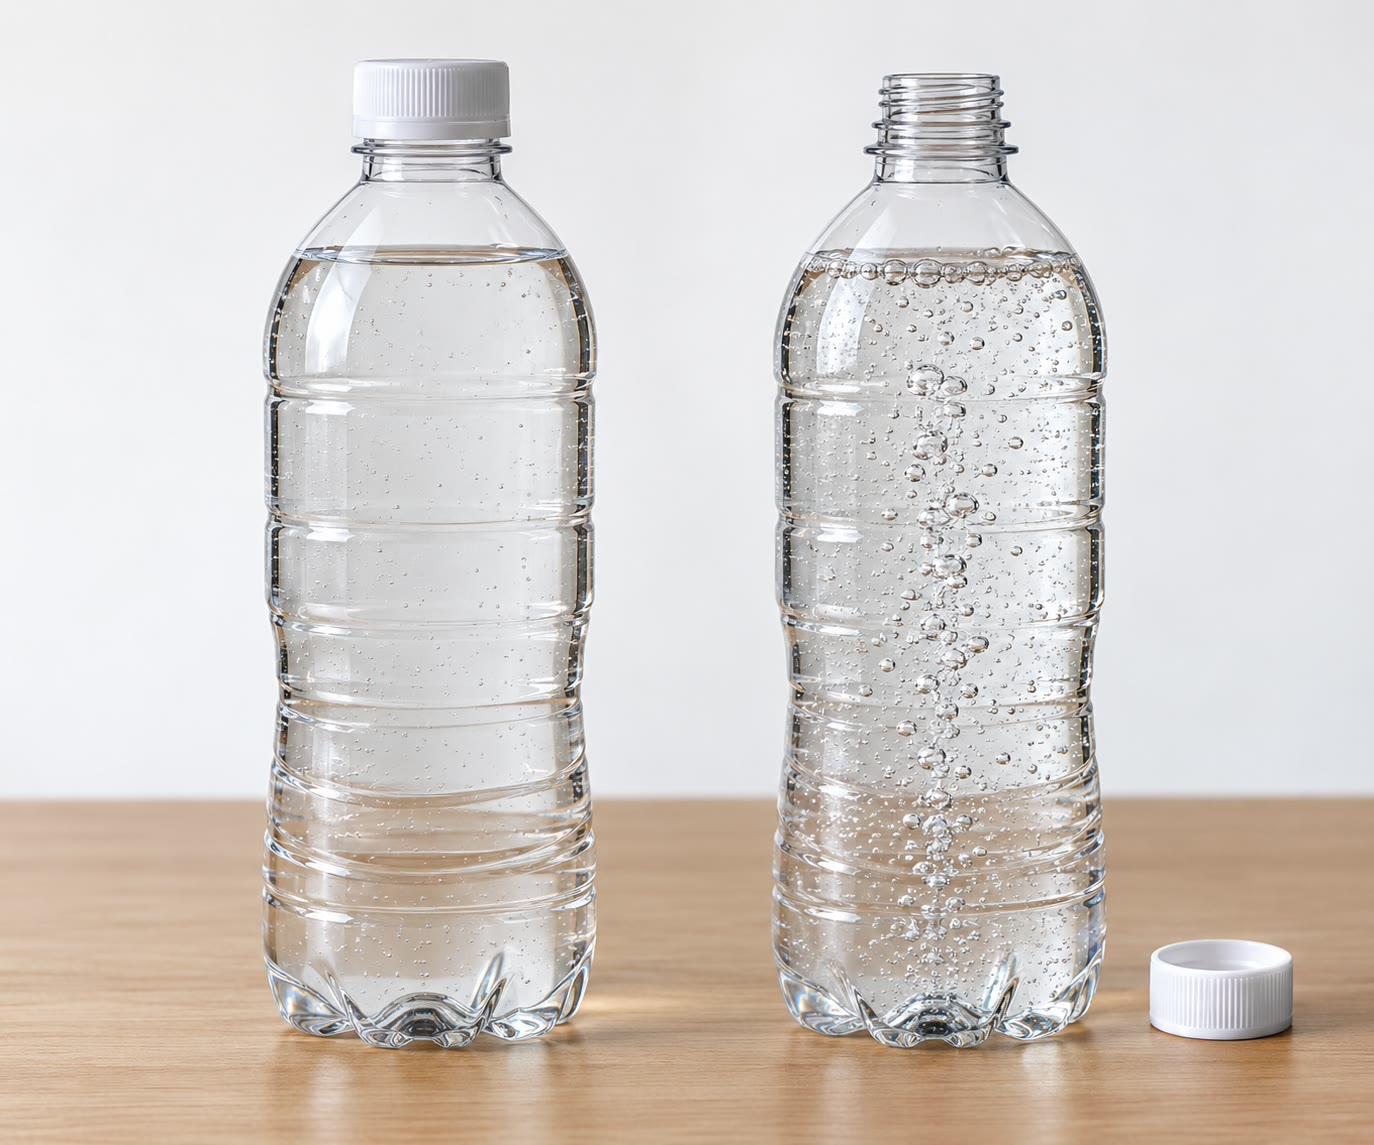
\includegraphics[width=0.45\linewidth,height=5cm,keepaspectratio]{images/book1/ai/g12-fizzy-bottles.jpg}

{\small Sealed, the water keeps its gas; opened, the gas escapes and does
not come back.}
\end{omfigure}

\section{Reactions that are not total}

\begin{definition}[Non-total reaction, final extent ratio]\label{def:g12:equilibrium:non-total}
A reaction is a \emph{non-total reaction}\index{non-total reaction} if it
stops at a final extent $x_f$ smaller than its \omterm{def:g10:reaction-progress-table:limiting}{maximum extent} $x_{\max}$,
with all the \omterm{def:g7:chemical-reactions:reactant}{reactants} still present. Its \emph{final extent
ratio}\index{final extent ratio} is
\[
  \tau = \frac{x_f}{x_{\max}}, \qquad 0 < \tau < 1
\]
($\tau = 1$ for a \omterm{def:g10:reaction-progress-table:limiting}{total reaction}).
\end{definition}

\begin{example}[An ester that stops halfway]\label{ex:g12:equilibrium:berthelot}
% ledger: ester:berthelot
Heated with \qty{1}{mol} of ethanol, \qty{1}{mol} of ethanoic acid forms
ethyl ethanoate and water,
\ce{CH3COOH + C2H5OH <=> CH3COOC2H5 + H2O}. The reaction stops when about
two thirds of the acid have reacted: $x_f = \qty{0.67}{mol}$ for
$x_{\max} = \qty{1}{mol}$, so $\tau \approx 0.67$. Starting from
\qty{1}{mol} of \omterm{def:g11:functional-groups:carboxylic-acid}{ester} and \qty{1}{mol} of water, the reverse reaction
also stops, with about one third of the \omterm{def:g11:functional-groups:carboxylic-acid}{ester} hydrolysed: the same final
\omterm{def:g6:pure-substances-and-mixtures:mixture}{mixture}.
\end{example}

\begin{history}[Berthelot and Péan de Saint-Gilles, 1862]
% ledger: ester:berthelot
The chemists Marcellin Berthelot and Léon Péan de Saint-Gilles heated
\omterm{def:g6:pure-substances-and-mixtures:mixture}{mixtures} of ethanoic acid and ethanol, and of ethyl ethanoate and water,
for long periods, and analysed them. From equal amounts of acid and
\omterm{def:g11:functional-groups:alcohol}{alcohol}, the reaction always stopped at about two thirds; from \omterm{def:g11:functional-groups:carboxylic-acid}{ester} and
water, at one third of hydrolysis; and they noticed that the amount of
\omterm{def:g11:functional-groups:carboxylic-acid}{ester} formed at each moment depended on the product of the amounts of
the \omterm{def:g7:chemical-reactions:reactant}{reactants}. Their work was one of the first quantitative studies of a
chemical equilibrium.
\end{history}

\section{The equilibrium state}

\begin{definition}[Equilibrium state]\label{def:g12:equilibrium:equilibrium-state}
A system is in an \emph{equilibrium state}\index{equilibrium state} when
its composition no longer changes although both the forward and the
reverse reactions are still going on, at the same rate. A reaction that
can reach such a state is written with the double arrow $\rightleftharpoons$.
\end{definition}

\begin{omfigure}
\begin{tikzpicture}
\begin{axis}[width=0.8\linewidth, height=6cm, xmin=0, xmax=200, ymin=0,
    ymax=1.05, xlabel={$t$ (\si{h})}, ylabel={amount of ester (\si{mol})},
    axis lines*=left, ymajorgrids, grid style={gray!20},
    tick label style={font=\small}, label style={font=\small},
    legend style={font=\small, at={(0.98,0.98)}, anchor=north east,
    draw=none, fill=white}, legend cell align=left]
  % ledger: ester:berthelot (K = 4; kinetics synthetic)
  \addplot[very thick, omDef] table[x=t, y=fromAcid] {figdata/out/grade-12-equilibrium.dat};
  \addplot[very thick, omProp] table[x=t, y=fromEster] {figdata/out/grade-12-equilibrium.dat};
  \addplot[dashed, black!60] coordinates {(0,0.6667) (200,0.6667)};
  \legend{from 1 mol acid + 1 mol alcohol, from 1 mol ester + 1 mol water}
  \node[font=\small, anchor=north east] at (axis cs:195,0.65) {equilibrium: $\tfrac{2}{3}$ mol};
\end{axis}
\end{tikzpicture}

{\small The esterification (blue) and the hydrolysis of the \omterm{def:g11:functional-groups:carboxylic-acid}{ester}
(orange) reach the same equilibrium composition, from opposite sides.
(The time scale is a model; the final value is the measured one.)}
\end{omfigure}

\section{The reaction quotient}

\begin{notation}[Standard concentration]\label{not:g12:equilibrium:c-standard}
$c^\circ = \qty{1}{mol/L}$ is the standard concentration. Dividing a
concentration by $c^\circ$ gives a number without unit with the same
value: $[\ce{A}]/c^\circ$.
\end{notation}

\begin{definition}[Reaction quotient]\label{def:g12:equilibrium:quotient}
For a reaction in solution $a\,\ce{A} + b\,\ce{B} \rightleftharpoons c\,\ce{C} + d\,\ce{D}$, the \emph{reaction
quotient}\index{reaction quotient} in a given state of the system is
\[
  Q = \frac{\left([\ce{C}]/c^\circ\right)^c \left([\ce{D}]/c^\circ\right)^d}
           {\left([\ce{A}]/c^\circ\right)^a \left([\ce{B}]/c^\circ\right)^b} .
\]
Solids, and the \omterm{def:g6:solutions-and-solubility:solute}{solvent} (water in an \omterm{def:g6:solutions-and-solubility:solute}{aqueous solution}), do not appear in
$Q$.
\end{definition}


\begin{example}[Writing quotients]\label{ex:g12:equilibrium:quotients}
For \ce{CH3COOH + H2O <=> CH3COO- + H3O+} in water (the \omterm{def:g9:ions:ion}{ion} \ce{H3O+} is
introduced in the next chapter), water is the \omterm{def:g6:solutions-and-solubility:solute}{solvent}:
$Q = \dfrac{[\ce{CH3COO-}]\,[\ce{H3O+}]}{[\ce{CH3COOH}]\,c^\circ}$. For the
dissolving of a solid, \ce{AgCl(s) <=> Ag+ + Cl-}, the solid is left out:
$Q = [\ce{Ag+}][\ce{Cl-}]/(c^\circ)^2$. For the esterification, where all
four species are in the same liquid \omterm{def:g6:pure-substances-and-mixtures:mixture}{mixture} of volume $V$, the volumes
cancel and $Q = \dfrac{n_{\text{ester}}\, n_{\text{water}}}{n_{\text{acid}}\, n_{\text{alcohol}}}$.
\end{example}

\section{The equilibrium constant}

\begin{definition}[Equilibrium constant]\label{def:g12:equilibrium:constant}
The value $Q_{eq}$ of the \omterm{def:g12:equilibrium:quotient}{reaction quotient} in the \omterm{def:g12:equilibrium:equilibrium-state}{equilibrium state} is
the \emph{equilibrium constant}\index{equilibrium constant} $K$ of the
reaction. It has no unit.
\end{definition}

\begin{proposition}[$K$ depends only on the temperature]\label{prop:g12:equilibrium:constant}
For a given reaction, $Q_{eq} = K$ in every \omterm{def:g12:equilibrium:equilibrium-state}{equilibrium state} at a given
temperature, whatever the initial amounts.
\end{proposition}

\begin{proof}
Admitted; it is derived in the Year 2 volume. It is checked on the
esterification: both runs of the figure, started from opposite sides,
give the same $Q_{eq}$.
\end{proof}

\begin{example}[$K$ of the esterification]\label{ex:g12:equilibrium:k-ester}
% ledger: ester:berthelot
From \qty{1}{mol} of acid and \qty{1}{mol} of \omterm{def:g11:functional-groups:alcohol}{alcohol}, the equilibrium
holds $\frac{2}{3}$ mol of \omterm{def:g11:functional-groups:carboxylic-acid}{ester} and of water and $\frac{1}{3}$ mol of
acid and of \omterm{def:g11:functional-groups:alcohol}{alcohol}:
\[
  K = \frac{(2/3)\times(2/3)}{(1/3)\times(1/3)} = 4 .
\]
\end{example}

\begin{method}[Final state of a non-total reaction]\label{met:g12:equilibrium:final}
\begin{enumerate}
  \item Fill the \omterm{def:g10:reaction-progress-table:extent}{progress table} with the unknown final extent $x_f$.
  \item Write $Q_{eq}$ as a function of $x_f$ and set it equal to $K$.
  \item Solve for $x_f$ (often a quadratic equation), keeping the root
        between 0 and $x_{\max}$.
  \item Deduce the final amounts and $\tau = x_f/x_{\max}$.
\end{enumerate}
\end{method}

\begin{example}[An excess of alcohol]\label{ex:g12:equilibrium:excess}
From \qty{1}{mol} of acid and \qty{2}{mol} of \omterm{def:g11:functional-groups:alcohol}{alcohol}:
$\dfrac{x^2}{(1-x)(2-x)} = 4$, that is $3x^2 - 12x + 8 = 0$, whose root
between 0 and 1 is $x_f = \qty{0.845}{mol}$. Doubling the \omterm{def:g11:functional-groups:alcohol}{alcohol} raises
the \omterm{def:g10:synthesis-yield:yield}{yield}, counted on the acid, from \qty{67}{\percent} to
\qty{85}{\percent}.
\end{example}

\section{Predicting and shifting the evolution}

\begin{proposition}[Direction of evolution]\label{prop:g12:equilibrium:direction}
If $Q < K$, the system evolves in the forward direction (the products
increase) until $Q = K$; if $Q > K$, it evolves in the reverse direction;
if $Q = K$, it is in equilibrium and does not change.
\end{proposition}

\begin{proof}
Admitted: $Q$ increases when the forward reaction proceeds (products in
the numerator grow, \omterm{def:g7:chemical-reactions:reactant}{reactants} in the denominator shrink), and the system
moves towards the state where $Q = K$.
\end{proof}

\begin{omfigure}
\begin{tikzpicture}[font=\small]
  \draw[->, thick] (0,0) -- (10,0) node[right] {$Q$};
  \draw[thick] (0,-0.12) -- (0,0.12) node[above] {0};
  \draw[very thick, omThm] (5,-0.25) -- (5,0.25) node[above] {$K$};
  \draw[->, very thick, omDef] (1.2,0.55) -- (4.4,0.55);
  \node[omDef, align=center] at (2.8,1.15) {$Q < K$: forward};
  \draw[->, very thick, omProp] (8.8,0.55) -- (5.6,0.55);
  \node[omProp, align=center] at (7.2,1.15) {$Q > K$: reverse};
  \node[align=center] at (5,-0.75) {$Q = K$: equilibrium};
\end{tikzpicture}

{\small The quotient always moves towards the constant.}
\end{omfigure}

\begin{remark}[Shifting an equilibrium]\label{rem:g12:equilibrium:shift}
To obtain more product from a \omterm{def:g12:equilibrium:non-total}{non-total reaction}, one can add an excess
of one \omterm{def:g7:chemical-reactions:reactant}{reactant} (the cheaper one), or remove a product as it forms: each
makes $Q < K$ again, and the system moves forward. Removing the water of
an esterification (with a drying agent, or by distilling it off) can
drive the reaction almost to completion. The open bottle of sparkling
water does the same with the carbon dioxide that escapes.
\end{remark}

\begin{omfigure}
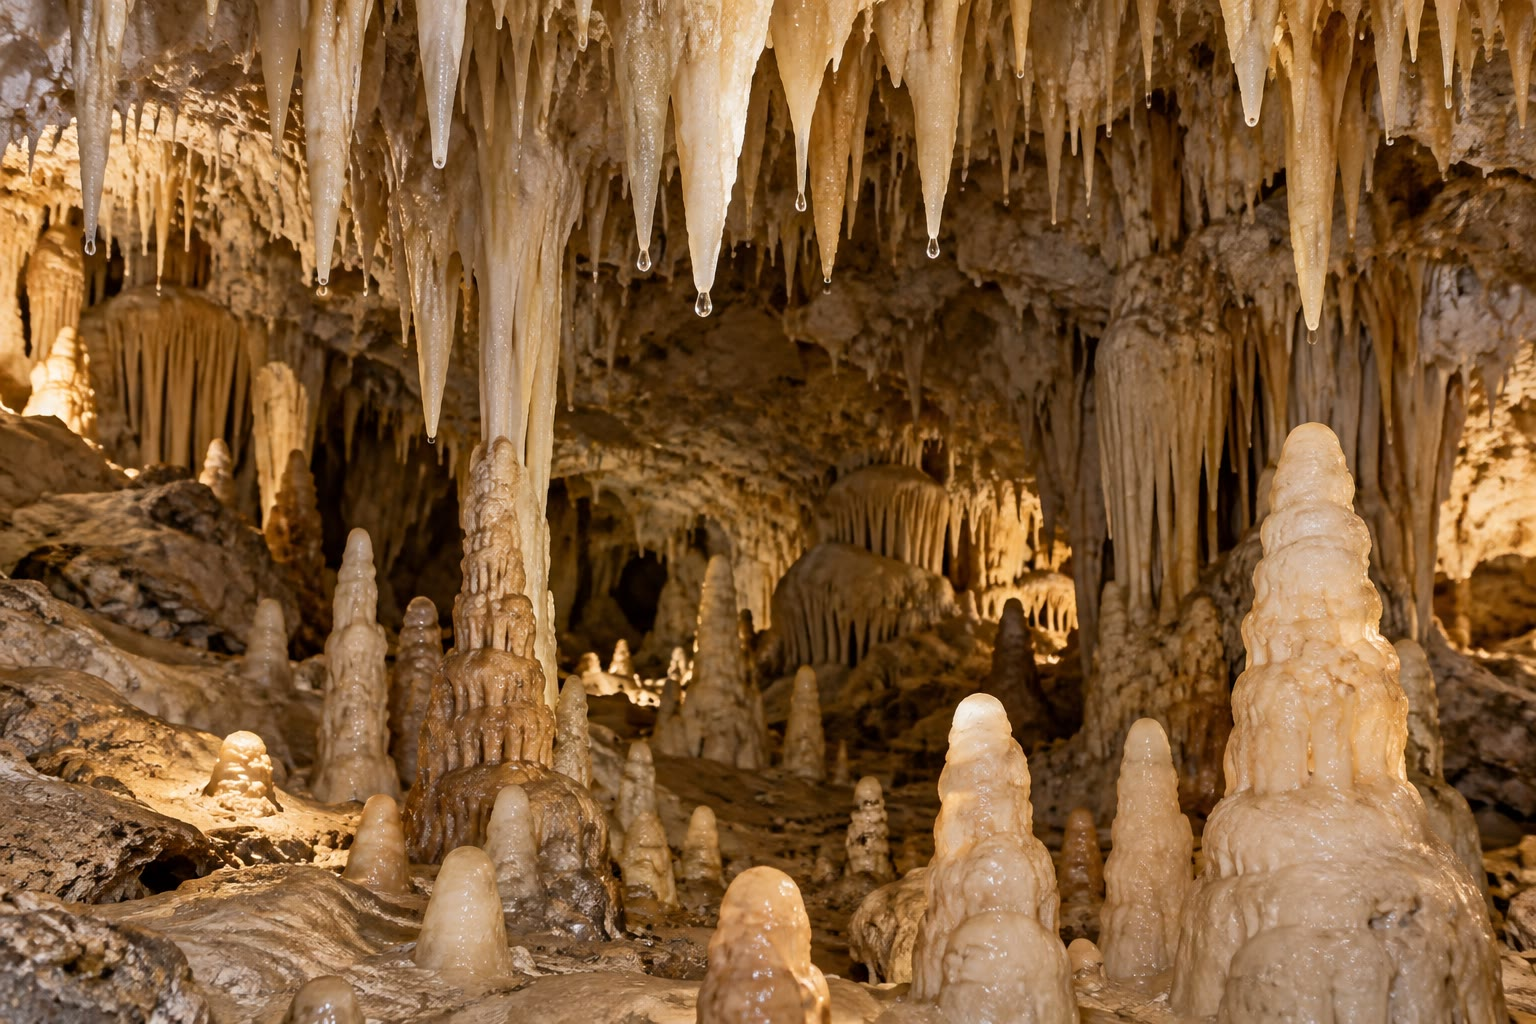
\includegraphics[width=0.45\linewidth]{images/book1/ai/g12-cave-stalactites.jpg}

{\small Stalactites grow where water dripping in a cave loses carbon
dioxide to the \omterm{def:g4:air-a-mixture-of-gases:air}{air}: an equilibrium of dissolved limestone is shifted, and
calcium carbonate is deposited.}
\end{omfigure}

\section{Exercises}

\begin{exercise}[$\star$]\label{exo:g12:equilibrium:1}
Write the \omterm{def:g12:equilibrium:quotient}{reaction quotient} of: (a) \ce{N2 + 3H2 <=> 2NH3} (gases, use
concentrations); (b) \ce{CH3COOH + H2O <=> CH3COO- + H3O+} in water;
(c) \ce{CaCO3(s) <=> Ca^{2+} + CO3^{2-}}; (d) \ce{Fe^{3+} + SCN- <=>
FeSCN^{2+}}.
\end{exercise}

\begin{exercise}[$\star$]\label{exo:g12:equilibrium:2}
A reaction has $x_{\max} = \qty{0.050}{mol}$ and reaches
$x_f = \qty{0.020}{mol}$. Compute $\tau$. Is the reaction total?
\end{exercise}

\begin{exercise}[$\star$]\label{exo:g12:equilibrium:3}
For a reaction with $K = 10$, in which direction does a \omterm{def:g6:pure-substances-and-mixtures:mixture}{mixture} evolve if
$Q = 2$? If $Q = 50$? If $Q = 10$?
\end{exercise}

\begin{exercise}[$\star$]\label{exo:g12:equilibrium:4}
Explain why an equilibrium is said to be ``dynamic''.
\end{exercise}

\begin{exercise}[$\star$]\label{exo:g12:equilibrium:5}
Does a \omterm{def:g12:catalysis:catalyst}{catalyst} change $K$? The time needed to reach equilibrium? Explain.
\end{exercise}

\begin{exercise}[$\star\star$]\label{exo:g12:equilibrium:6}
\qty{2.0}{mol} of ethanoic acid and \qty{2.0}{mol} of ethanol are mixed
($K = 4$). Compute the final amounts of the four species.
\end{exercise}

\begin{exercise}[$\star\star$]\label{exo:g12:equilibrium:7}
A \omterm{def:g6:pure-substances-and-mixtures:mixture}{mixture} contains \qty{0.5}{mol} each of ethanoic acid, ethanol, ethyl
ethanoate and water. Compute $Q$. In which direction does it evolve?
\end{exercise}

\begin{exercise}[$\star\star$]\label{exo:g12:equilibrium:8}
Using the figure of the two runs, read the amount of \omterm{def:g11:functional-groups:carboxylic-acid}{ester} after
\qty{20}{h} in each run. When can the system be considered at
equilibrium?
\end{exercise}

\begin{exercise}[$\star\star$]\label{exo:g12:equilibrium:9}
Starting from \qty{1}{mol} of \omterm{def:g11:functional-groups:carboxylic-acid}{ester} and \qty{1}{mol} of water ($K = 4$
for the esterification, so $1/4$ for the hydrolysis), compute the final
amounts by the method of the chapter, and compare with the esterification
run.
\end{exercise}

\begin{exercise}[$\star\star$]\label{exo:g12:equilibrium:10}
Why does the solid not appear in the quotient of
\ce{AgCl(s) <=> Ag+ + Cl-}? Does adding more solid shift the
equilibrium?
\end{exercise}

\begin{exercise}[$\star\star$]\label{exo:g12:equilibrium:11}
In a closed bottle of sparkling water, carbon dioxide leaves and enters
the water at the same rate. Write the equilibrium
\ce{CO2(aq) <=> CO2(g)} and explain, with $Q$ and $K$, why the water goes
flat when the bottle is opened.
\end{exercise}

\begin{exercise}[$\star\star\star$]\label{exo:g12:equilibrium:12}
An esterification of \qty{1}{mol} of acid and \qty{1}{mol} of \omterm{def:g11:functional-groups:alcohol}{alcohol}
reaches equilibrium. Half of the water present is then removed. Compute
the new $Q$, say in which direction the system evolves, and find the new
final amount of \omterm{def:g11:functional-groups:carboxylic-acid}{ester}.
\end{exercise}

\begin{exercise}[$\star\star\star$]\label{exo:g12:equilibrium:13}
Show that the constant of the reverse reaction is $1/K$. What is the
constant of the hydrolysis of ethyl ethanoate?
\end{exercise}

\begin{exercise}[$\star\star\star$]\label{exo:g12:equilibrium:14}
A chemist \omterm{def:g2:mixing-and-dissolving:mix}{mixes} \qty{1}{mol} of acid, \qty{1}{mol} of \omterm{def:g11:functional-groups:alcohol}{alcohol},
\qty{2}{mol} of \omterm{def:g11:functional-groups:carboxylic-acid}{ester} and \qty{0.5}{mol} of water. Will anything happen?
Explain.
\end{exercise}

\begin{exercise}[$\star\star\star$]\label{exo:g12:equilibrium:15}
What excess of \omterm{def:g11:functional-groups:alcohol}{alcohol} (amount per \omterm{def:g10:the-mole:amount}{mole} of acid) is needed to esterify
\qty{95}{\percent} of the acid? Solve $\dfrac{0.95^2}{0.05(n - 0.95)} =
4$.
\end{exercise}

\section{Problem: Berthelot's Ester}

\begin{problem}[{Weekend problem --- how much ester when the alcohol is
put in threefold excess?}]
\label{pb:g12:equilibrium:1}
% ledger: ester:berthelot, aw:C, aw:H, aw:O
Ethyl ethanoate, a \omterm{def:g6:solutions-and-solubility:solute}{solvent} and a flavouring, is made from ethanoic acid
and ethanol. In 1862 Berthelot and Péan de Saint-Gilles found that from
equal amounts of acid and \omterm{def:g11:functional-groups:alcohol}{alcohol} the reaction stops when about two thirds
of the acid have reacted.

\medskip
\noindent\textbf{Part I --- The reaction.}
\begin{enumerate}
  \item Write the equation of the esterification, with \omterm{def:g11:organic-skeletons:formulas}{semi-structural
        formulas}.
  \item Why is it written with a double arrow?
  \item Write its \omterm{def:g12:equilibrium:quotient}{reaction quotient} in amounts.
  \item From \qty{1}{mol} of acid and \qty{1}{mol} of \omterm{def:g11:functional-groups:alcohol}{alcohol}, what is
        $x_{\max}$? What is $x_f$, from Berthelot's result?
  \item Compute $\tau$.
\end{enumerate}

\medskip
\noindent\textbf{Part II --- The constant.}
\begin{enumerate}[resume]
  \item Give the final amounts of the four species.
  \item Compute $K$.
  \item Starting from \qty{1}{mol} of \omterm{def:g11:functional-groups:carboxylic-acid}{ester} and \qty{1}{mol} of water,
        Berthelot found one third hydrolysed. Show that this agrees with
        the same $K$.
  \item Why must $K$ be the same in both cases?
\end{enumerate}

\medskip
\noindent\textbf{Part III --- A threefold excess of \omterm{def:g11:functional-groups:alcohol}{alcohol}.}
\begin{enumerate}[resume]
  \item From \qty{1}{mol} of acid and \qty{3}{mol} of \omterm{def:g11:functional-groups:alcohol}{alcohol}, fill the
        \omterm{def:g10:reaction-progress-table:extent}{progress table}.
  \item Write the equation $Q_{eq} = K$ and show that it becomes
        $3x^2 - 16x + 12 = 0$.
  \item Solve it, and keep the meaningful root.
  \item What fraction of the acid is esterified?
  \item Compute the mass of \omterm{def:g11:functional-groups:carboxylic-acid}{ester} obtained.
\end{enumerate}

\medskip
\noindent\textbf{Part IV --- Removing water.}
\begin{enumerate}[resume]
  \item From the equimolar equilibrium, the water is removed as it
        forms. Explain with $Q$ why the reaction goes on.
  \item If all the water could be removed, what would the \omterm{def:g10:synthesis-yield:yield}{yield} become?
  \item Why is the \omterm{def:g11:functional-groups:alcohol}{alcohol}, not the acid, usually put in excess? (Think
        of the cost and of separating the products.)
  \item Does heating the \omterm{def:g6:pure-substances-and-mixtures:mixture}{mixture} change the \omterm{def:g10:reaction-progress-table:system}{final state}, or only the
        time to reach it? (The esterification gives out almost no heat.)
  \item State the final answer: what fraction of the acid is esterified
        with a threefold excess of \omterm{def:g11:functional-groups:alcohol}{alcohol}?
\end{enumerate}
\end{problem}
